\documentclass[10pt,a4paper,oneside]{article}
\usepackage[latin1]{inputenc}
\usepackage{amsmath}
\usepackage{amsfonts}
\usepackage{amssymb}
\usepackage{graphicx} 

\title{ Simple \LaTeX\ Paper}
\author{Manrique Salas,Brenda }
\date{"23 de Noviembre de 2010"} 

\begin{document}
\maketitle


\section*{Resumen}\begin{flushright}
\begin{flushright}
\begin{flushright}
\begin{flushright}
\begin{flushright}
\begin{flushright}
\end{flushright}
\end{flushright}
\end{flushright}
\end{flushright}
\end{flushright}
\end{flushright}
Las bases de datos distribuidas se desarrollaron para que la informaci\'on sea compartida por distintos usuarios y los datos sean utilizados desde distintos sitios, siendo la caracter\'istica m\'as importante la transparencia de los procesos. Este sistema involucra diferentes objetivos los cuales generan diversos problemas los que no permiten un sistema de bases de datos distribuida ideal. Adem\'as se trata el concepto de middleware para la comunicaci\'on entre los tipos de bases de datos.

\section*{Palabras Claves}
Sistemas Distribuidos, Bases de Datos Distribuidas, DBMS.

\section*{Abstract}
The distributed databases are developed to ensure that information is shared by several users and the data are used from different places, being transparency of processes the most important characteristic. Although this system involves different objectives that drive the use of such database, we’ll see that sometimes they generate different problems from getting an ideal system for distributed databases. In addition we talk about the concept of middleware for communication between the types of databases.


\section*{Key Words}
Distributed Systems, Distributed Database, DBMS.


\section{Introducci\'on}
\\\\Desde los a\~nos 70 se almacenaba la informaci\'on de manera centralizada, pero con el paso del tiempo las necesidades aumentaron y esto produjo ciertos inconvenientes que no era posible solucionarlos o volverlos eficientes de la forma centralizada. Estos problemas impulsaron la creaci\'on de almacenamiento distribuido, los cuales hoy en d\'ia proveen caracter\'isticas indispensables en el manejo de informaci\'on; es decir, la combinaci\'on de las redes de comunicaci\'on y las bases de datos.
\\\\Seg\'un \cite{Hernandez} Una BDD es en realidad un tipo de base de datos virtual cuyas partes componentes est\'an almacenadas en varias de datos reales que se encuentran en varias sitios distintos, en otras palabras es la uni\'on l\'ogica de esas bases de datos reales.

\section{Definici\'on}
\\\\Seg\'un \cite{Date} "El soporte completo para las bases de datos distribuidas implica que una sola aplicaci\'on debe ser capaz de operar de manera transparente sobre los datos que est\'an dispersos en una variedad de bases de datos diferentes, administradas por una variedad de distintos DBMSs, ejecutadas en diversas m\'aquinas diferentes, conectadas a una variedad de redes de comunicaci\'on distintas; donde el t\'ermino de {\bf manera transparente} significa que la aplicaci\'on opera desde un punto de vista l\'ogico como si todos los datos fueran manejados por un solo DBMS y ejecutados en una sola m\'aquina."
\\\\Se considera una base de datos distribuida a aquellas que cumplen lo siguiente:
\begin {itemize}
\item Los datos deben estar f\'isicamente en m\'as de un sitio.
\item Los sitios deben estar interconectadas.
\item Los datos han de estar l\'ogicamente integrados. 
\item En una \'unica operaci\'on se puede acceder (recuperar o actualizar) datos que se encuentran en m\'as de un sitio.
\item Todas las acciones que necesiten realizarse sobre m\'as de un sitio ser\'an transparentes al usuario.
\end {itemize}
\\\\Cada sitio local contiene:
\begin {itemize}

\item Sus propias bases de datos reales.
\item Sus propios usuarios locales.
\item Su propio DBMS local.
\item Su propia administraci\'on de datos locales.
\end {itemize}
\begin {figure} [¡h]
\centering
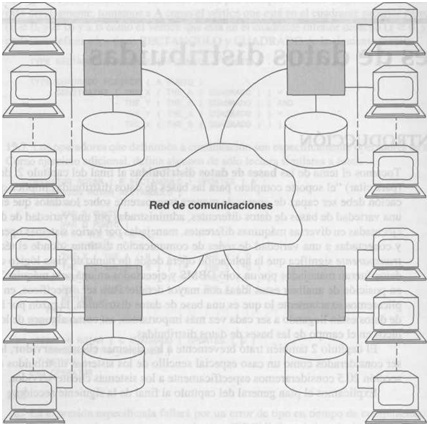
\includegraphics [width=0.4 \textwidth] {fig1}
\caption {Ejemplo BDD t\'ipica}
\label {fig:fig1}
\end {figure}

\\\\Un BDD es bastante conveniente pero a la vez m\'as complicado, es por ello que diversos fabricantes y desarrolladores dedican gran esfuerzo en la implementaci\'on de este servicio cada vez mejor.
\\\\Es importante distinguir entre sistemas de bases de datos distribuidas {\bf verdaderos y generalizados}, de los sistemas que simplemente proporcionan alg\'un tipo de acceso a datos remotos (que son en realidad sistemas cliente-servidor).
\\\\En un {\bf sistema de acceso a datos remotos}, el usuario puede operar simult\'aneamente sobre datos que est\'an en un sitio remoto o incluso en varios sitios remotos de los cuales se est\'a definitivamente consciente, de alguna manera, de que los datos son remotos; por el contrario, en un {\bf verdadero sistema de base de datos distribuida} es totalmente transparente al usuario.
\\\\Existen dos tipos de transacciones. Tenemos las {\bf transacciones locales}, que se dan cuando se accede a un \'unico sitio remoto, y las {\bf transacciones globales} las que recopilan datos de diferentes sitios.
\\\\Las bases de Datos Distribuidas utilizan la t\'ecnica de {\bf r\'eplica de datos}, que est\'a basada en la copia de datos de disco a disco, donde existe un gestor de replicas que las administra para un mejor rendimiento, disponibilidad y tolerancia a fallos, las que trabajan de manera transparente y coherente. Esto involucra la {\bf propagaci\'on de la actualizaci\'on} que no es nada m\'as que actualizar todas las copias de un objeto replicado.
\\\\Tambi\'en se da la {\bf Fragmentaci\'on de Datos} que divide los datos en varios sitios de los cuales son obtenidos mediante transacciones globales. Existen b\'asicamente dos tipos de fragmentaci\'on, {\bf horizontal y vertical}, que corresponden a las operaciones relaci\'onales de {\bf restricci\'on y proyecci\'on}, respectivamente.
\\\\Se distinguen dos tipos de sistemas, un {\bf sistema homog\'eneo} donde las DBMS son las mismas  y resulta m\'as flexible la administraci\'on; adem\'as de un {\bf sistema heterog\'eneo} donde se trabaja con diferentes DBMS (p.e MySQL, PostgreSQL, etc.) lo que significa relacionar todas estas para su distribuci\'on.



\section{Ventajas\cite {Olarte}}
\begin {itemize}
\item {\bf Flexibilidad y fiabilidad}, acceso desde distintos lugares y por distintas personas a la vez sin inconvenientes.
\item Mejora del {\bf rendimiento}, BD m\'as peque\~nas, operaciones de menor volumen.
\item {\bf Compartimiento de datos}. Los usuarios de un sitio son capaces de acceder a los datos de uno o m\'as sitios.
\item {\bf Autonom\'ia}. Cada sitio tiene cierto grado de control sobre sus datos.
\item {\bf Disponibilidad}. Si en un sistema distribuido falla un sitio, los sitios restantes pueden seguir funcionando. Si se duplican los datos en varios sitios, la transacci\'on que necesite un determinado dato puede encontrarlo en cualquiera de los diferentes sitios.
\end {itemize}


\section{Desventajas\cite {Olarte}}
\begin {itemize}
\item {\bf Coste de desarrollo del software}. La complejidad a\~nadida que es necesaria para mantener la coordinaci\'on entre nodos hace que el desarrollo de software sea m\'as costoso.
\item {\bf Mayor probabilidad de errores}. Como los nodos que constituyen el sistema funcionan en paralelo, es m\'as dif\'icil asegurar el funcionamiento correcto de los algoritmos, as\'i como de los procedimientos de recuperaci\'on de fallos del sistema.
\item {\bf Mayor sobrecarga de procesamiento}. El intercambio de mensajes y ejecuci\'on de algoritmos para el mantenimiento de la coordinaci\'on entre sitios supone una sobrecarga que no se da en los sistemas centralizados.



\section{Un principio fundamental}
El principio fundamental de la base de datos distribuida segun \cite{Date}
\\"Ante el usuario, un sistema distribuido debe lucir exactamente igual que un sistema que no es distribuido"\\
Un sistema distribuido debe ser capaz de comportarse exactamente como si el sistema no fuera distribuido. Todos los problemas de los sistemas distribuidos son, o deber\'ian ser, problemas internos o en el nivel de implementaci\'on, y no externos o en el nivel del usuario.
\\Este principio nos conduce a doce reglas complementarias \\

\subsection{Autonom\ía local}

Los sitios en un sistema distribuido deben ser aut\'onomos.
\\Idealmente la autonom\'ia local significa que las operaciones de un sitio X no debe depender de alg\'un otro sitio Y. Los datos locales son pose\'idos y administrados localmente. Por lo tanto, la seguridad, integridad y representaci\'on de almacenamiento de los datos locales permanecen bajo el control y jurisdicci\'on del sitio local.
\\\\Sin embargo este concepto no es totalmente alcanzable, existen varias situaciones en las que un sitio X dado debe transferir un determinado grado de control a alg\'un otro sitio Y. Por lo tanto, el objetivo de autonom\'ia queda establecido con mayor precisi\'on como: los sitios deben ser aut\'onomos en el mayor grado posible
\\\\Aqu\'i resumimos algunas situaciones: 
\begin{itemize}
\item Normalmente, no es posible acceder directamente a fragmentos individuales de una VR fragmentada, ni siquiera desde el sitio en el que est\'an almacenados.
\item Normalmente, no es posible acceder directamente a copias individuales de una VR  replicada (o fragmentada), ni siquiera desde el sitio en el que est\'an almacenadas.
\item Sea P la copia primaria de alguna VR R replicada (o fragmentada), y sea que P est\'a almacenada en el sitio X. Entonces, todo sitio que acceda a R es dependiente del sitio X, aunque otra copia de R est\'a de hecho almacenada en el sitio en cuesti\'on.
\item No es posible acceder a una VR que participa en una restricci\'on de integridad de varios sitios, para efectos de actualizaci\'on, dentro del contexto local del sitio en el que est\'a almacenada, sino s\'olo dentro del contexto de la base de datos distribuida en el que est\'a definida la restricci\'on.
\item Un sitio que est\'a actuando como participante en un proceso de confirmaci\'on de dos fases, debe obrar de acuerdo a las decisiones (es decir confirmar o deshacer) del sitio coordinador correspondiente.
\end{itemize}
\subsection{No dependencia de un sitio central}
La autonom\'ia local implica que todos los sitios deben ser tratados como iguales. Por lo tanto, no debe haber particularmente ninguna dependencia de un sitio "maestro" central para alg\'un servicio central. 
\\La dependencia de un sitio central ser\'ia indeseable por las siguientes dos razones
\begin{itemize}
\item Primero, el sitio central puede ser un cuello de botella. 
\item Segundo y m\'as importante, el sistema ser\'ia vulnerable; es decir, si el sitio central falla, tambi\'en fallar\'a todo el sistema
\end{itemize}
\subsection{Operaci\'on contin\'ua}
En general, una ventaja de los sistemas distribuidos es que deben proporcionar mayor confiabilidad y mayor disponibilidad.
\begin{itemize}
\item La confiabilidad (es decir, la probabilidad de que el sistema est\'a listo y funcionando en cualquier momento dado) Los sistemas distribuidos pueden continuar operando (en un nivel reducido) cuando hay alguna falla en alg\'un componente independiente
\item La disponibilidad (es decir, la probabilidad de que el sistema est\'a listo y funcionando continuamente a lo largo de un per\'iodo especificado) tambi\'en mejora, en parte por la misma raz\'on y en parte debido a la posibilidad de replicaci\'on de datos
\end{itemize}
\subsection{Independencia de ubicaci\'on}
Los usuarios no tienen que saber d\'onde est\'an almacenados f\'isicamente los datos, sino que deben ser capaces de comportarse al menos desde un punto de vista l\'ogico como si todos los datos estuvieran almacenados en su propio sitio local.
\\La independencia de ubicaci\'on es necesaria debido a que simplifica los programas de usuario y las actividades terminales
\subsection{Independencia de fragmentaci\'on}
Un sistema soporta la fragmentaci\'on de datos cuando una VR dada puede ser dividida en partes o fragmentos, para efectos de almacenamiento f\'isico. 
\\La fragmentaci\'on es necesaria por razones de rendimiento: los datos pueden estar almacenados en la ubicaci\'on donde son usados m\'as frecuentemente para que la mayor\'ia de las operaciones sean locales y se reduzca el tr\'afico en la red. 
\begin{figure}[!h]
  \centering
    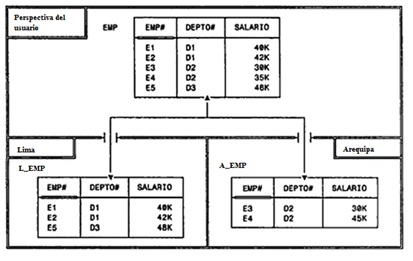
\includegraphics[width=0.4\textwidth]{fig2}
  \caption{Fragmentaci\'on horizontal 1}
  \label{fig:fig2}
\end{figure}
\\Por ejemplo, considere una VR de empleados EMP con los valores de ejemplo que muestra la parte superior de la figura ~\ref{fig:fig2} En un sistema que soporta la fragmentaci\'on, podr\'iamos definir dos fragmentos de la siguiente forma:
\\FRAGMENT EMP AS
\\L\_ EMP AT SITE 'Lima' WHERE DEPTO $=$ 'D1' OR DEPTO $=$ 'D3';
\\A\_ EMP AT SITE 'Arequipa' WHERE DEPTO $=$ 'D2';
\\\\La reconstrucci\'on de la VR original a partir de los fragmentos es lograda por medio de las operaciones de junta y de uni\'on adecuadas (junta para los fragmentos verticales y uni\'on para los horizontales). 
\\La facilidad de fragmentaci\'on y la facilidad de reconstrucci\'on son dos de las razones principales por las que los sistemas distribuidos son relacionales; el modelo relacional proporciona exactamente las operaciones necesarias para estas tareas 
\\La independencia de fragmentaci\'on implica que a los usuarios se les presentar\'a una vista de los datos en la cual los fragmentos estar\'an recombinados l\'ogicamente por medio de juntas y de uniones adecuadas. Es responsabilidad del optimizador del sistema determinar cu\'ales fragmentos necesitan ser accedidos f\'isicamente para satisfacer cualquier solicitud de usuario dada. Por ejemplo, dada la fragmentaci\'on que muestra la figura si el usuario hace la solicitud
\\EMP WHERE SALARIO $>$ 40K AND DEPTO $=$ 'D1'
\\El optimizador sabr\'a, por medio de las definiciones de fragmentos (guardadas en el cat\'alogo, por supuesto), que el resultado completo puede ser obtenido desde el sitio de Lima; no hay necesidad de acceder al sitio de Arequipa.
\\\\La VR EMP, tal como es percibida por el usuario, puede ser considerada (aproximadamente) como una vista de los fragmentos subyacentes L\_ EMP y A\_ EMP:
\\VAR EMP VIEW 
\\L\_ EMP UNION A\_ EMP;
\\\\El optimizador transforma entonces la solicitud original del usuario en lo siguiente:
\\ (L\_ EMP UNION A\_ EMP ) WHERE SALARIO $>$ 40K AND DEPTO  'D1?
\\\\Esta expresi\'on puede ser transformada todav\'ia m\'as en:
\\(L\_ EMP WHERE SALARIO $>$ 40K AND DEPTO $=$ 'D1')
\\UNION 
\\(A \_ EMP WHERE SALARIO $>$ 40K AND DEPT0 $=$ 'D1')
\\\\A partir de la definici\'on del fragmento A\_ EMP en el cat\'alogo, el optimizador sabe que el segundo de estos dos operandos de UNION da como resultado una relaci\'on vac\'ia 
\\\\La expresi\'on general puede entonces ser simplificada a s\'olo
\\L\_ EMP WHERE SALARIO $>$ 40K AND DEPTO $=$ 'D1'
\\Ahora el optimizador sabe que necesita acceder solamente al sitio de Lima

\subsection{Independencia de replicaci\'on}
Un sistema soporta la replicaci\'on de datos cuando una VR almacenada puede ser representada por muchas copias distintas, o r\'eplicas, guardadas en muchos sitios distintos. 
\\Las r\'eplicas son necesarias por dos razones (como m\'inimo). 
\begin{itemize}
\item Rendimiento (las aplicaciones pueden operar sobre copias locales en lugar de tener que comunicarse con sitios remotos). 
\item Fiabilidad(al haber m\'ultiples copias de los datos disponibles en el sistema, se dispone de un mecanismo excelente de recuperaci\'on cuando existan fallos en sitios).
\end{itemize}

\begin{figure}[!h]
  \centering
    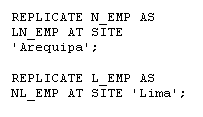
\includegraphics[width=0.4\textwidth]{fig4}
  \caption{Ejemplo}
  \label{fig:fig4}
\end{figure}
\begin{itemize}
\item Desventaja: al actualizar un objeto replicado es necesario actualizar todas las copias de ese objeto (propagaci\'on de la actualizaci\'on).
\item La replicaci\'on debe ser "transparente ante el usuario". 
\item Un sistema que soporta la replicaci\'on de datos tambi\'en debe soportar la independencia de replicaci\'on es necesaria debido a que simplifica los programas de usuario y las actividades terminales; en particular, permite que las r\'eplicas sean creadas y destruidas en cualquier momento en respuesta a los distintos requerimientos, sin invalidar ninguno de esos programas de usuario o actividades.
\item  La independencia de replicaci\'on implica que es responsabilidad del optimizador del sistema determinar cu\'ales r\'eplicas necesitan ser accedidas f\'isicamente para satisfacer cualquier solicitud de usuario dada. 
\end{itemize}
\begin{figure}[!h]
  \centering
    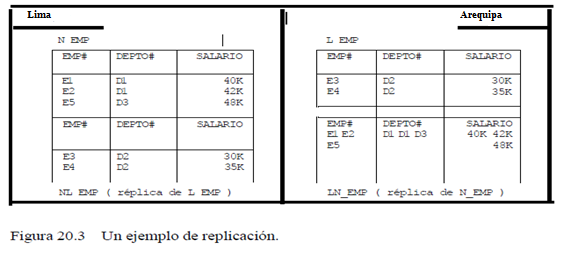
\includegraphics[width=0.4\textwidth]{fig3}
  \caption{Ejemplo}
  \label{fig:fig3}
\end{figure}

\subsection{Procesamiento de consultas distribuidas}
La optimizaci\'on es importante en un sistema distribuido.
\\El punto b\'asico es que en una consulta que involucra a varios sitios, habr\'a muchas formas posibles de mover los datos en el sistema para satisfacer la solicitud, y es crucialmente importante que se encuentre una estrategia eficiente. 

\subsection{Administraci\'on de transacciones distribuidas}
Hay dos aspectos principales en la administraci\'on de transacciones: el control de la recuperaci\'on y el control de la concurrencia. 
\\Una transacci\'on es manejada por varios agentes, donde la ejecuci\'on de c\'odigo puede ser ejecutada en muchos sitios y un agente es el proceso realizado en nombre de una transacci\'on en un sitio dado.
\\El sistema necesita saber cu\'ando dos agentes son parte de la misma transacci\'on (por ejemplo, para no caer en bloqueo).
\\Recuperaci\'on: para asegurarse de que una transacci\'on dada sea at\'omica en el ambiente distribuido, el sistema debe por lo tanto asegurarse de que el conjunto de agentes para esa transacci\'on sea confirmado o deshecho al un\'isono. 
\\Control de concurrencia: el control de concurrencia est\'a basado generalmente en el bloqueo. 

\subsection{Independencia de hardware}
Soporte para un gran n\'umero de m\'aquinas diferentes. Poder integrar todos los datos de todos estos sistemas y presentar al usuario una "imagen del sistema \'unico".
\subsection{Independencia de sistema operativo}
Es necesario tener la posibilidad de ejecutar el mismo DBMS en diferentes plataformas de sistema operativo.
\subsection{Independencia de red}
Si el sistema va a tener la posibilidad de soportar muchos sitios distintos es obviamente necesario tener la posibilidad de soportar tambi\'en una variedad de redes de comunicaci\'on distintas. 
\subsection{Independencia de DBMS}
Lo que se necesita es que todos los ejemplares de DBMS en sitios diferentes soporten la misma interfaz.
\begin{itemize}

\item Aunque no tienen que ser necesariamente copias del mismo software DBMS.
\item En otras palabras, ser\'ia posible que el sistema distribuido fuera heterog\'eneo, al menos en cierto grado.
\item Ser\'ia muy bueno si diferentes DBMS pudieran participar de alguna forma en un sistema distribuido. 
\end{itemize}


\section{Problemas}
\subsection{Procesamiento de consultas}
\subsection{Administraci\'on de cat\'alogo}


\subsection{Propagaci\'on de actualizaci\'on}
\\\\El problema en la replicaci\'on de datos es que una actualizaci\'on a cualquier objeto debe ser propagada a todas las copias almacenadas de ese objeto. 
\\\\Una dificultad es que si un sitio que mantiene una copia del objeto no est\'a disponible en el momento de la actualizaci\'on, debido a una falla del sitio o de la red, esta transacci\'on fallar\'ia.  Esto debilita a una de las ventajas que mencionamos anteriormente.
\\\\Una soluci\'on a este problema es el esquema de {\bf copia primaria}, que funciona de la siguiente forma:
\begin {itemize}
\item A una copia de cada objeto replicado se le designa como copia primaria. Todas las dem\'as
son copias secundarias.
\item Las copias primarias de diferentes objetos est\'an en diferentes sitios.
\item Cuando se actualiza la copia primaria, el sitio que mantiene esa copia es responsable de la propagaci\'on de la actualizaci\'on hacia las copias secundarias. 
\end {itemize}


\subsection{Control de recuperaci\'on}
\\\\El control de la recuperaci\'on en sistemas distribuidos est\'a basado t\'ipicamente en el protocolo  de  {\bf confirmaci\'on de dos fases}. La confirmaci\'on de dos fases nos permite, no solo reconstruir lo que sucedi\'o justo antes del   fallo, sino que protege a los nodos que no han fallado para que no lean los datos que representan un estado inconsistente\cite{Pastor}.
\\\\La confirmaci\'on de dos fases se da cuando una transacci\'on interacciona con varios gestores aut\'onomos con el prop\'osito de asegurar que todos los gestionadores de recursos relativos a esta transacci\'on la aceptaran toda o bien la rechazaran, garantizando que la transacci\'on sea todo o nada\cite{Pastor}.

\subsection{Control de la concurrencia}
\\\\El control de concurrencia requiere mucho estudio, pero a pesar de esto no hay ning\'un algoritmo aceptado para solucionar el problema\cite{Carzola}. Esto se debe a varios factores de los cuales se consideran a los siguientes tres los m\'as determinantes:
\begin {enumerate}
\item La data puede estar duplicada. por tanto, el manejador  es responsable de localizar y actualizar la data duplicada.
\item Si un sitio falla o la comunicaci\'on con un sitio falla mientras se realiza una actualizaci\'on, el manejador debe asegurarse de que los efectos se reflejen una vez el sitio se recupere del fallo.
\item La sincronizaci\'on de transacciones en sitios m\'ultiples es dif\'icil ya que estos no pueden obtener informaci\'on inmediata de las acciones realizadas en otros sitios concurrentemente.
\end {enumerate}

\\\\El ejemplo m\'as com\'un de un bloqueo mutuo es cuando un recurso A est\'a siendo utilizado por una transacci\'on A que a su vez solicita un recurso B que est\'a siendo utilizado por una transacci\'on B que solicita el recurso A. Entre los ejemplos espec\'ificos para las bases de datos distribuidas podemos destacar:
\begin {itemize}
\item Actualizaci\'on perdida: cuando dos transacciones concurrentes borran sus actualizaciones.
\item La extracci\'on inconsistente: acceder a informaci\'on modificada parcialmente por una transacci\'on.
\end {itemize}

\\\\Para el control de bloqueos mutuos no se ha desarrollado ninguna soluci\'on viable y la forma m\'as simple y que la mayor\'ia de productos utilizan es la implementaci\'on de un tiempo m\'aximo de espera en las peticiones de bloqueos.



\section{Independencia de DBMS}
\\\\Regresando uno  de los doce objetivos para los sistemas de bases de datos distribuidos en general. La suposici\'on de homogeneidad estricta es discutible; todo lo que en realidad necesitamos es que los DBMSs que est\'an en sitios diferentes soporten la misma interfaz. Por ejemplo, MySQL y Oracle soportan el est\'andar oficial de SQL deber\'ia ser posible hacer que se comportaran en sociedad dentro de un sistema distribuido heterog\'eneo
\\\\ {\bf Pasarela}
\\\\Para que 2 o m\'as DBMS de comuniquen se debe proporcionar un programa especial, llamado pasarela, su funci\'on es hacer que los DBMSs se parezcan". Como lo indica la Figura 1.
\\
\begin {figure} [¡h]
\centering
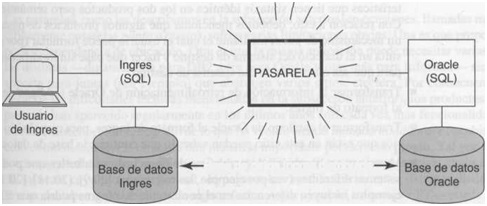
\includegraphics [width=0.4 \textwidth] {figx}
\caption {Una pasarela hipot\'etica proporcionada por Ingres para Oracle}
\label {fig:figx}
\end {figure}
\\\\Implementar los protocolos para intercambiar informaci\'on entre diferentes DBMSs implica transformar el formato de mensaje en el cual son enviadas las instrucciones fuente.
\\\\En otras palabras, la {\bf pasarela} debe ser capaz de ejecutar cualquier instrucci\'on SQL no planeada en un tipo de Base de Datos. 
\\\\Hacer transformaciones entre los tipos de datos de cada DBMS incluyen subproblemas ya que tienen que ver con situaciones tales como las diferencias en el procesador,  las diferencias en el c\'odigo de caracteres, las diferencias en el formato de punto flotante, etc\'etera.
\\\\Transformar la informaci\'on de retroalimentaci\'on de Oracle (c\'odigos de retorno, etc\'etera) al formato de Ingres.
\\\\Transformar el cat\'alogo de Oracle al formato de Ingres, para que el sitio Ingres y los usuarios que est\'an en este sitio puedan saber lo que contiene la base de datos Oracle.
\\\\Servir como participante en (la variante de Ingres para) el protocolo de confirmaci\'on de dos fases (suponiendo que se permita que las transacciones de Ingres realicen actualizaciones en la base de datos Oracle). La posibilidad de que la pasarela realice esta funci\'on, depender\'a de las propiedades proporcionadas por el administrador de transacciones en el sitio.

\\\\ {\bf Middleware para acceso a datos}
\\\\Las pasarelas, sufren varias limitaciones. Una es que proporcionan poca independencia de ubicaci\'on. Otra es que la misma aplicaci\'on puede necesitar varias pasarelas distintas, p.e. una para PostgreSQL, otra para Oracle y otra m\'as para MySQL. 
\\\\Por consecuencia, los productos del tipo pasarela han aparecido regularmente en los \'ultimos a\~nos con cada vez m\'as funcionalidad sofisticada. De hecho, todo el negocio de lo que ha venido siendo llamado middleware (tambi\'en conocido como mediadores) es ahora una industria importante. 
\\\\Los middleware se adaptan a las diferentes plataformas para su correcto funcionamiento y para que todo proceso se realice de manera transparente de tal manera que no importe que sistema operativo se utilice, la comunicaci\'on se realiza con total flexibilidad. 


\section{Conclusiones}
\begin {itemize}
\item En este documento se ha intentado dado una visi\'on general de los problemas y caracter\'isticas de una base de datos distribuida. Se ha tocado el tema de las t\'ecnicas de fragmentaci\'on horizontal y vertical, las t\'ecnicas son sencillas y son de f\'acil el entendimiento.

\item Adem\'as, est\'an apareciendo m\'etodos de fragmentaci\'on mixta como el que se ha comentado. Si bien, estos m\'etodos son enfoques formales m\'as que pr\'acticos, aun siendo desarrollados.

\item Los sistemas gesti\'on de base de datos distribuidos heterog\'eneas son una realidad que a\'un est\'an limitados por la experiencia actual. Tambi\'en necesitan seguir afrontando distintos entornos y variaciones durante un tiempo

\item Pese a la aparici\'on de los m\'etodos de bases de datos distribuidas hace ya a\~nos, parece que el salto de lo centralizado a lo distribuido a escala comercial est\'a por venir. Todav\'ia no se ha extendido suficientemente el esquema distribuido, pero se espera que pr\'oximamente se produzca el avance definitivo.

\item Considerando los dos componentes b\'asicos de los sistemas de bases de datos distribuidos (la propia base de datos y la red de ordenadores) y adem\'as, la situaci\'on actual de la inform\'atica. Si las bases de datos es una de las ramas m\'as antiguas e importantes de la inform\'atica, muchas empresas compran ordenadores para dedicarlos exclusivamente a la gesti\'on de sus datos, como parece ser que se ha asumido por parte de todo tipo de empresarios los beneficios que acarrea la conexi\'on de los ordenadores, la instalaci\'on de una red, se puede concluir diciendo que el terreno ya est\'a abonado para su extensi\'on comercial. 

\item S\'olo hace falta que determinadas multinacionales decidan apostar m\'as fuerte por este enfoque a trav\'es de sus famosos sistemas gestores de bases de datos y que se produzca la consolidaci\'on de la resoluci\'on de los problemas que el enfoque distribuido acarrea.
\end {itemize}

%BIBLIOGRAFIA 
\include{bibliografia}
%FIN DE LA BIBLIOGRAFIA
\end{document}
\end{document}